% From Template LaTeX file for DAFx-11 papers
%
% To generate the correct references using BibTeX, run latex, bibtex, latex, latex

\def\papertitle{Nonlinear Allpass Ladder Filters in Faust}
\def\paperauthorA{Julius O. Smith}
\def\paperauthorB{Romain Michon}

\documentclass[twoside,a4paper]{article}
\usepackage{dafx_11}
\usepackage{amsmath,amssymb,amsfonts,amsthm}
\usepackage{euscript}
\usepackage[latin1]{inputenc}
\usepackage[T1]{fontenc}
\usepackage{ifpdf}

\usepackage[english]{babel}
\usepackage{caption}
\usepackage{subfig, color}

\setcounter{page}{1}
\ninept

\usepackage{times}
% Saves a lot of ouptut space in PDF... after conversion with the distiller
% Delete if you cannot get PS fonts working on your system.

% pdf-tex settings: detect automatically if run by latex or pdflatex
\newif\ifpdf
\ifx\pdfoutput\relax
\else
   \ifcase\pdfoutput
      \pdffalse
   \else
      \pdftrue
\fi

\ifpdf % compiling with pdflatex
  \usepackage[pdftex,
    pdftitle={\papertitle},
    pdfauthor={\paperauthorA, \paperauthorB},
    colorlinks=false, % links are activated as colror boxes instead of color text
    bookmarksnumbered, % use section numbers with bookmarks
    pdfstartview=XYZ % start with zoom=100% instead of full screen; especially useful if working with a big screen :-)
  ]{hyperref}
  \pdfcompresslevel=9
  \usepackage[pdftex]{graphicx}
  \usepackage[figure,table]{hypcap}
\else % compiling with latex
  \usepackage[dvips]{epsfig,graphicx}
  \usepackage[dvips,
    colorlinks=false, % no color links
    bookmarksnumbered, % use section numbers with bookmarks
    pdfstartview=XYZ % start with zoom=100% instead of full screen
  ]{hyperref}
  % hyperrefs are active in the pdf file after conversion
  \usepackage[figure,table]{hypcap}
\fi

\title{\papertitle}

\affiliation{
\paperauthorA\mbox{ and }\paperauthorB\sthanks{CCRMA visiting researcher from Saint \'Etienne University, France, supported by the ASTREE Project}}
{\href{https://ccrma.stanford.edu/\~{}jos/}{Center for Computer Research in Music and Acoustics}\\ (CCRMA) Stanford University \\ Palo Alto, CA 94305, USA\\
{\tt \href{mailto:jos|rmichon@ccrma.stanford.edu}{jos@ccrma.stanford.edu}}
}

\newcommand{\zi}{z^{-1}}
\begin{document}
% more pdf-tex settings:
\ifpdf % used graphic file format for pdflatex
  \DeclareGraphicsExtensions{.png,.jpg,.pdf}
\else  % used graphic file format for latex
  \DeclareGraphicsExtensions{.eps}
\fi

\maketitle

\begin{abstract}
Passive nonlinear filters provide a rich source of evolving spectra
for sound synthesis.  This paper describes ...

\end{abstract}

\section{Introduction}
\label{sec:intro}

Many musical instruments have important nonlinear effects influencing
their sound.  In particular, cymbals and gongs exhibit evolving
spectra due to nonlinear coupling among their resonant modes
\cite{FletcherAndRossing98}.  One effective method for efficiently
synthesizing such sounds is using the digital waveguide mesh
\cite{vanDuy93,sav00} terminated by nonlinear allpass filters
\cite{PierceAndVanDuyne97}.  The mesh models linear wave propagation
in 2D, while the nonlinear allpass provides nonlinear coupling of the
modes of vibration in a way that conserves signal energy, and
therefore does not affect damping (which is introduced via lowpass
filters at selected points in the mesh).  Thus, nonlinear allpass
filters provide a valuable tool for nonlinear mode combination while
preserving stability and keeping decay-time separately controllable.

\section{Passive Nonlinear Filters}

\subsection{First-Order Switching Allpass}

The passive nonlinear filter described in \cite{PierceAndVanDuyne97}
was based on the idea of terminating a vibrating string on two
different springs $k_1$ and $k_2$, as shown in Fig.{}
\ref{stringk1k2}.  The switching spring-constant creates a
nonlinearity in the string-spring system.  Importantly, the switching
from one spring to the other only accurs when the spring displacements
are zero, so that energy is not affected.  (The potential energy
stored in a spring $k_i$ displaced by $x_i$ meters is given by
$k_ix_i^2/2$ \cite{PASP}.)

\begin{figure}[ht]
\centerline{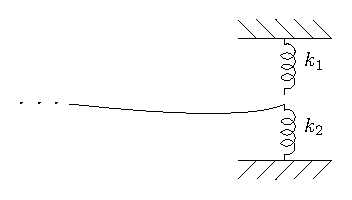
\includegraphics[scale=0.8]{eps/stringk1k2.eps}}
\caption{\label{stringk1k2}{\it Vibrating string terminated by two
    different springs $k_1$ and $k_2$. Only one spring is active at a
    time.}}
\end{figure}

In an ideal vibrating string with wave impedance $R$ \cite{PASP},
terminating the string by an ideal spring $k_i$ provides an
\emph{allpass reflectance} at the end of the string for traveling
waves.  That is, reflected displacement waves $y^-(t)$ at the
termination are related to the incident waves $y^+(t)$ by
\[
Y^-(s) = Y^+(s) H_i(s) 
\]
where $H_i(s)$ is the (Laplace-domain) transfer function of the allpass filter
\[
H_i(s) = \frac{s-k_i/R}{s+k_i/R}.
\]
Replacing the ideal string by a digital waveguide \cite{PASP} and 
digitizing the spring reflectance $H_i(s)$ via the bilinear transform
yields the digital reflectance
\[
H_i(z) = -\frac{a_i+\zi}{1+a_i\zi},\qquad a_i=\frac{k_i-2Rf_s}{k_i+2Rf_s}
\]
where $f_s$ denotes the sampling rate in Hz.  While the digital
reflectance remains an allpass filter due to properties of the
bilinear transform, energy conservation is only
approximately obtained, except when the allpass state variable happens
to be exactly zero when the coefficient $a_i$ is switched from $a_1$ to
$a_2$ or vice versa.

\subsection{Delay-Line Length Modulation}

Since allpass filters are fully characterized by their time-delay at
each frequency, the switching allpass of the previous section can be
regarded as a form of nonlinear delay-line length modulation in which
the delay line switches between two allpass-interpolated lengths
(different at each frequency in general).

Delay-line length modulation has been used previously to simulate
nonlinear string behavior.  For example, the length modulations due to
tension variations have been addressed \cite{TolonenEtAl00}.
Additionally, it has long been recognized that the highly audible
nonlinearity of the sitar is due to the continuous length modulation
caused by its curved bridge \cite{FletcherAndRossing98}.  Similarly,
the tambura nonlinearly modulates its string length between two
lengths via a cotton thread near the bridge
\cite{FletcherAndRossing98}.  In digital waveguide models such as
\texttt{Sitar.cpp} in the Synthesis Tool Kit (STK) \cite{STK4},
delay-line length is modulated without careful regard for energy
conservation; this normally works out fine in practice because
lengthening a delay-line is energy conserving when the new samples
are zero, and shortening the delay-line is typically a bit lossy
and never energy-creating.

\section{Nonlinear Allpasses of Arbitrary Order}

We propose to extend the nonlinear switching allpass in two ways:
\begin{enumerate}
\item Any order allpass can be used (not just first order).
\item Any kind of coefficient modulation can be used (not just
  switching between two values at zero crossings of some state).
\end{enumerate}
Our method is based on the Normalized Ladder Filter (NLF)
\cite{GrayAndMarkel75}. Such filters can be derived from digital
waveguide filters by using normalized traveling waves in place of
ordinary physical traveling waves \cite{PASP}, where the normalization
is chosen so that the square of the traveling-wave amplitude equals
the power associated with that sample throughout the waveguide
network.

Figure \ref{nlf} shows the first-order NLF allpass as it is typically
drawn \cite{MG,PASP}.

\begin{figure}[ht]
\centerline{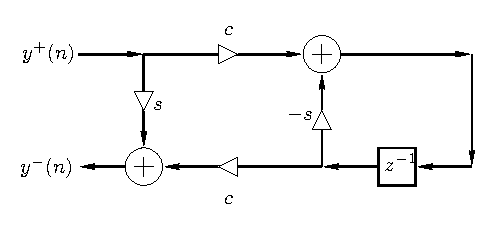
\includegraphics{eps/nlf.eps}}
\caption{\label{nlf}{\it First-order normalized ladder allpass filter, with
coefficients $c=\cos(\theta)$ and $s=\sin(\theta)$, $\theta\in[-\pi,\pi]$.}}
\end{figure}

Figure \ref{nlf1} shows the same filter as it is depicted in the block diagram
rendered by ``\texttt{faust -svg}'' for the Faust expression
%\begin{quote}
% {\small
\begin{verbatim}
process = 
   _ <: *(s),(*(c):(+:_)~(*(-s))):_,*(c)':+;
\end{verbatim}
% }
%\end{quote}
The function \texttt{allpassnn(1)} is equivalent to this in the Faust
distribution (\texttt{filter.lib} after 2/2/11).

% rsvg-convert --format=ps tapnnfig-svg/process.svg > nlf1.eps
\begin{figure}[ht]
\centerline{\includegraphics[scale=0.33]{eps/nlf1.eps}}
\caption{\label{nlf1}{\it First-order normalized ladder allpass filter as drawn by Faust.}}
\end{figure}

A general property of allpass filters is that each delay element can
be replaced by an allpass to produce another allpass (a
circle-to-circle conformal map of the transfer function).  If the
delay element in Fig.{} \ref{nlf} is replaced by itself at the output
of another first-order allpass of the same form (Fig.{} \ref{nlf}),
then a second-order NLF allpass is obtained.  This process is extended
to arbitrary orders by replacing the rightmost delay by a first-order
NLF allpass followed by a delay.  This same recursive construction
works also for the Kelly-Lochbaum ladder allpass, and the
two-multiply and one-multiply lattice structures \cite{MG,PASP}.

In Faust, NLF allpass filters of arbitrary order are conveniently
specified by means of the pattern matching facility:
\begin{samepage}
\begin{verbatim}
allpassnn(0,tv) = _;
allpassnn(n,tv) = _ <: *(s), (*(c) : 
  (+ : allpassnn(n-1,tv))~(*(-s))) 
  : _,*(c)':+
  with { 
    c=cos(take(n,tv));  s=sin(take(n,tv)); 
  };
\end{verbatim}
\end{samepage}
This is the full definition of \texttt{allpassnn()} in 
\texttt{filter.lib}.

Figure \ref{nlf2} shows the block diagram generated for the
second-order NLF allpass specified as \texttt{allpassnn(2,tv)}.

\begin{figure*}[ht]
\center
%\includegraphics[width=5in,bb=3 257 607 534]{eps/nlf2.eps}
\includegraphics[width=6.5in]{eps/nlf2.eps}
\caption{\label{nlf2}{\it Second-order NLF allpass as drawn by Faust.}}
\end{figure*} 

\section{Energy Invariance Illustration}

The following Faust program illustrates the energy-invariance property
of the normalized-ladder allpass for order 3:
\begin{verbatim}
import("filter.lib"); // for allpassnn
N = 3; // order desired
theta = par(i,N,PI*noise@(10*i+100));
rms = ^(2) : smooth(0.9999) : sqrt;
uvwnoise = sqrt(3)*noise; // unit variance
process =  uvwnoise <: _, allpassnn(N,theta) 
           : rms, rms;
\end{verbatim}
The figure plotted by \texttt{faust2octave} is shown in Figure
\ref{tapnn2}.  We see that the root-mean-square (RMS) level of the
input and output signals are almost identical.  Thus, when applied to
unit-variance white noise, the output signal (and in fact every
state-variable within the filter) is unit-variance white noise, even
when the filter coefficients are modulated over their maximum range by
uncorrelated white noise.

\begin{figure}[ht]
\center
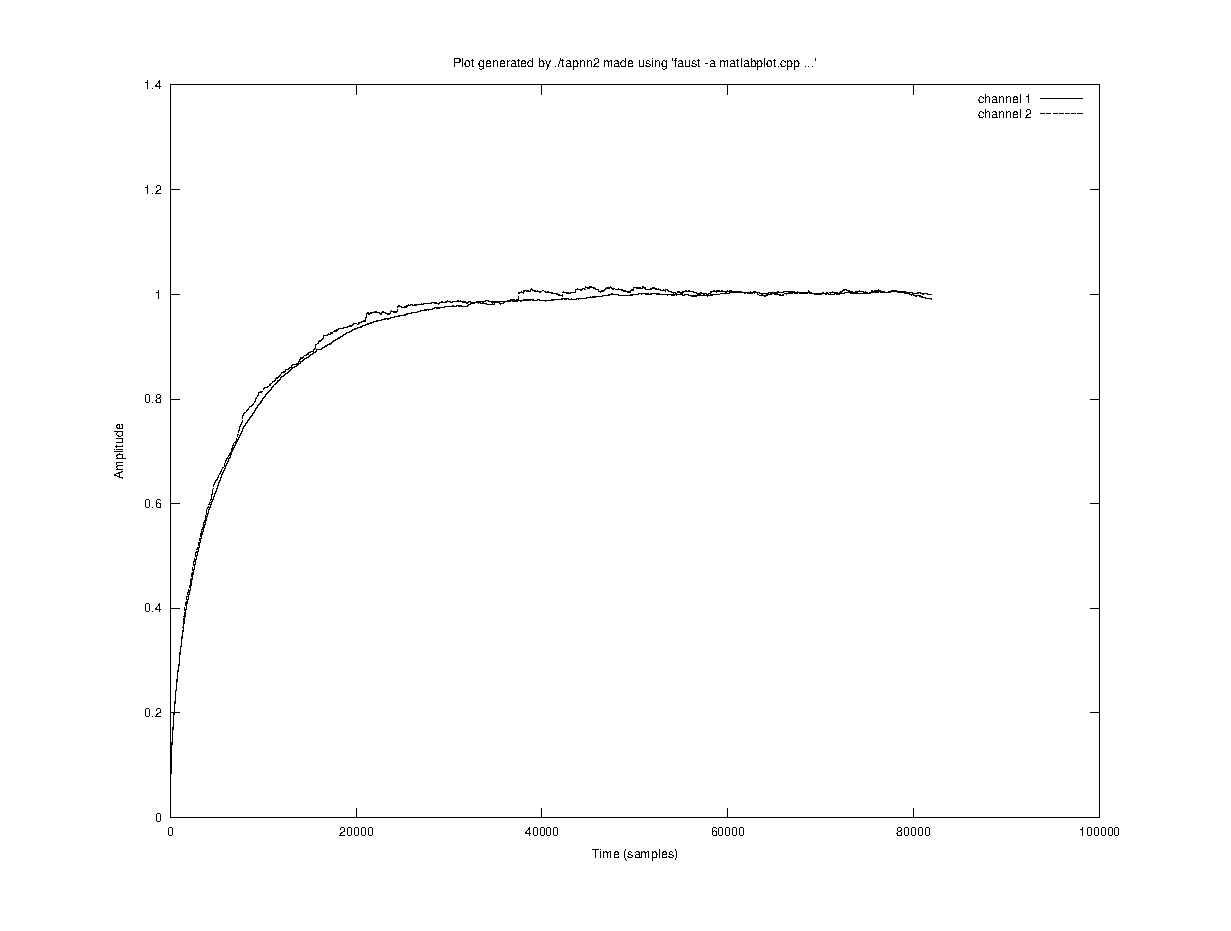
\includegraphics[width=3in]{eps/tapnn2.eps}
\caption{\label{tapnn2}{\it RMS level of input and output signals
for the third-order normalized-ladder allpass driven by white noise,
with uncorrelated white noise used as reflection coefficients.}}
\end{figure} 

It is interesting to note that if the reflection-coefficients are
instead computed using \verb!theta = par(i,N,PI*noise@(i+1));!, the
RMS level of the output signal rises somewhat \emph{above} that of the
input signal, as shown in Figure \ref{tapnn2tmc}.  Thus, correlations
between the input signal and the filter coefficients (as occurs in
nonlinear filtering applications0 can result in some power gain.
% 
% FIXME: SHOW THIS BETTER

\begin{figure}[ht]
\center
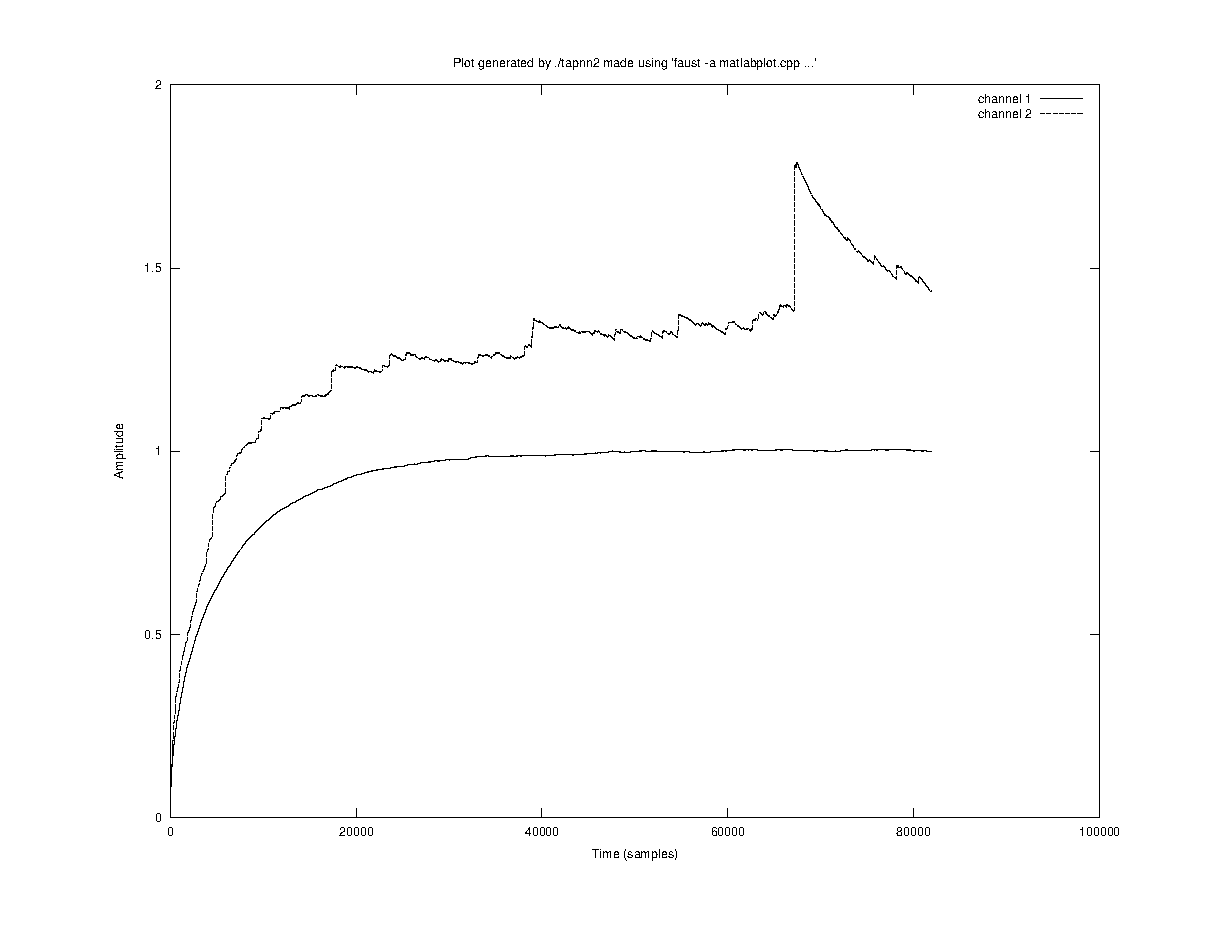
\includegraphics[width=3in]{eps/tapnn2tmc.eps}
\caption{\label{tapnn2tmc}{\it RMS level of input and output signals
for the third-order normalized-ladder allpass driven by white noise,
with weakly correlated white noise used as reflection coefficients.}}
\end{figure} 

As another interesting example, if the reflection-coefficients are
computed using \verb!theta = par(i,N,PI*noise);!, which means all
reflection coefficients vary together in lock-step with the input
noise, the RMS level of the output signal falls somewhat \emph{below}
that of the input signal, as shown in Figure \ref{tapnn2tc}.

\begin{figure}[ht]
\center
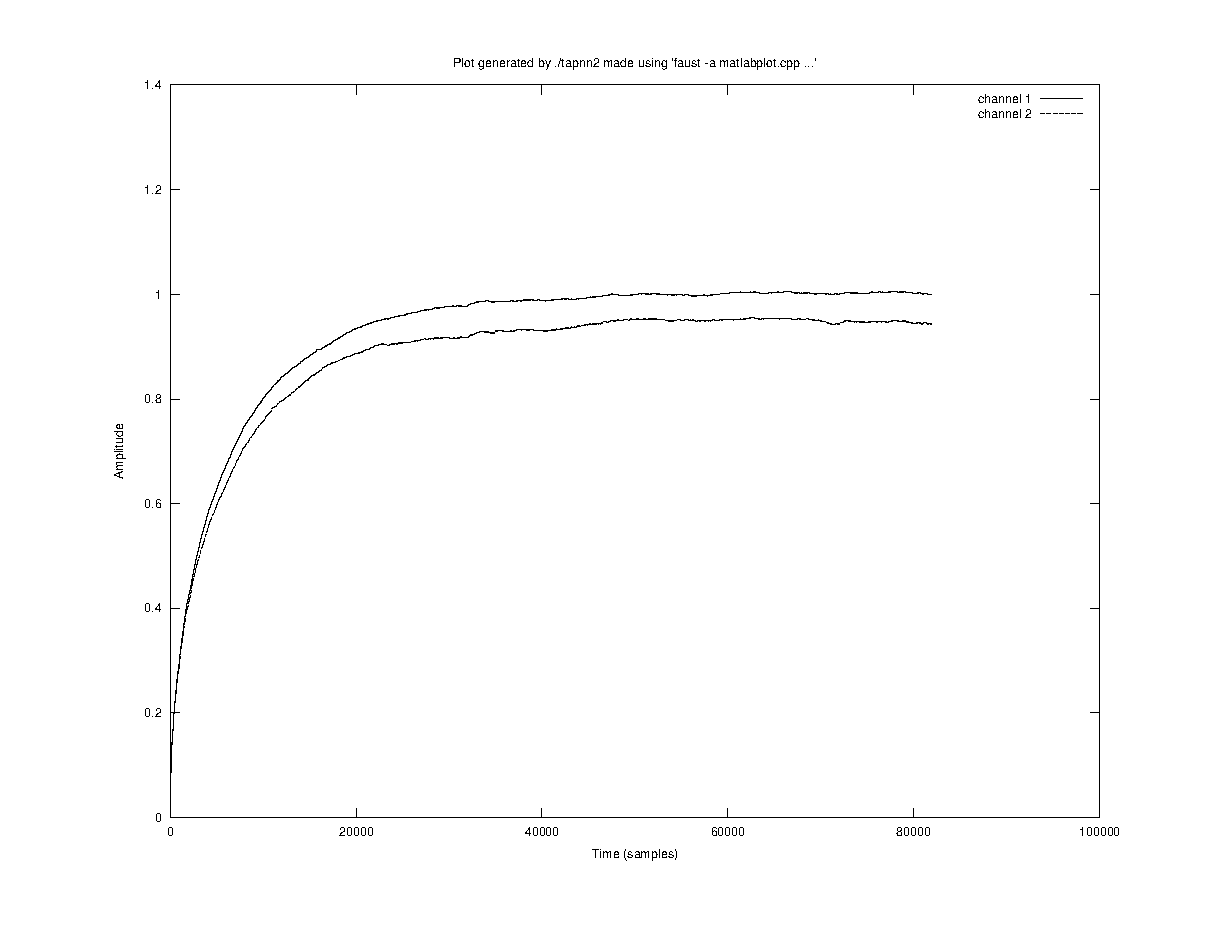
\includegraphics[width=3in]{eps/tapnn2tc.eps}
\caption{\label{tapnn2tc}{\it RMS level of input and output signals
for the third-order normalized-ladder allpass driven by white noise,
with the same white noise used as reflection coefficients.}}
\end{figure} 

\section{Conclusions}

\section{Acknowledgments}

%\newpage
{\small\raggedright
\nocite{*}
\bibliographystyle{IEEEbib}
\bibliography{dafx11-jos-rm}
}

\end{document}
